\chapter{Chapter One}
\section{Introduction}
Weather radar is an invaluable tool for hydrometeorological purposes; with the
refinement of operational polarimetric radars, it has become indispensable for
quantitative precipitation estimation (QPE). Numerous studies have shown the skill of
dual-pol estimators over traditional reflectivity-based algorithms, especially for
rainfall cases. One approach is using polarimetric moments directly in empirically derived power law relations. Previously,
two relations were developed by \cite{Hassan2017} ; one using just horizontal
reflectivity ($Z_H$), while the other incorporated differential reflectivity ($Z_{DR}$)
from the polarimetric C-Band radar at King City (CWKR). These algorithms were correlated
with ground measurements of snowfall accumulation.  The conclusion from the previous
dataset is that the addition of $Z_{DR}$ did not significantly improve the SWE
estimates, but both still performed better than the legacy algorithm used by Environment
Canada. Another approach for improving QPE estimates through polarimetric data is the
classification of hydrometeor types, then using a corresponding relation matched to that
type. While quantitative precipitation estimates contain statistical measurement error
propogated from $Z$ and $Z_{DR}$, this error is reduceable through spatial and temporal
smoothing. Meanwhile, smoothing will not remove biases in the moments. This error will
be propagated into QPE estimates, which is why its important to remove them. Here, it is
shown that with biased $Z_{DR}$ is used as input into Colorado State University
hydrometeor classification scheme, it is sucessful at filtering for similiar dry snow
targets in synoptic snowfall events with temperatures within the plate growth region,
while failing in lake-effect snow events. The purpose of the filtering is to yield
better estimates of systematic bias.
\section{Background}
First, it is important to provide some background on the weather radar moments that are presented in this study, from both single and dual polarized signals. The convention for representing these moments symbolically hereafter is lower-case subscript for linear units and upper-case subscript for logarithmic units, i.e. $Z_{DR}$ is logarithmic while $Z_{dr}$ is linear.
\subsection{Reflectivity Factor ($Z_{h}$)}
\begin{equation}\label{eq:ref_factor}
Z_{h} = \int_0^{\infty} N(D)D^6dD \ (mm^6/m^3)
\end{equation}
The foremost moment derived from radar is the reflectivity factor ($Z_{h}$), where the
subscript denotes its derivation from the horizontally polarized signal. This variable
measures the number density $N(D)$ of hydrometeors of diameter $D$ per unit volume, as
presented in Equation \ref{eq:ref_factor}. Due to uncertainties about what type of
target is actually doing the scattering, it is typically represented as the equivalent
reflectivity factor $Z_{eh}$, where $Z_{h}$ = $Z_{eh}$ if the targets are made of liquid 
water and are comparatively small to the wavelength \citep{Fabry2015}. The two names are 
essentially interchangeable, but the nomenclature $Z_{eh}$ will be used in this study to 
acknowledge the presence of non-ideal targets, e.g. snow crystals.
\subsection{Differential Reflectivity ($Z_{dr}$)}
Radars equipped with dual-polarimetric (dual-pol) capabilities are still an emerging technology, in terms of operational meteorological applications. These types of radar systems are capable of transmitting and receiving two orthogonally polarized electromagnetic waves in order to deduce more information about the microphysical structure of hydrometeors. One of the main variables this allows them to produce is $Z_{DR}$, defined as the ratio of the horizontal channel reflectivity ($Z_H$) to the vertical channel reflectivity $Z_{V}$). This can be simplified to the difference between the two using the logarithmic quotient rule, since they are represented in logarithmic units. Equation \ref{eq:zdr} demonstrates this concept.
\begin{equation}\label{eq:zdr}
Z_{dr} = 10 * \log_{10}(\frac{Z_H}{Z_V}) = Z_h - Z_h
\end{equation}
Although dual-pol radar has matured within the research community, operational deployment has been a much slower process. Many studies have been undertaken in regards to quantitative precipitation estimation using dual-pol variables for rainfall, but studies involving the estimation of snowfall liquid equivalent has been much more limited. In Canada, there is one active C-band weather radar with dual-pol capabilities. It is located north of Toronto, in King City, with rest of the network is currently undergoing an upgrade to polarimetric S-Band. Its neighbor to the south, KBUF, was upgraded to dual-pol in 2012 as part of a network wide upgrade. 
\begin{figure}[h]
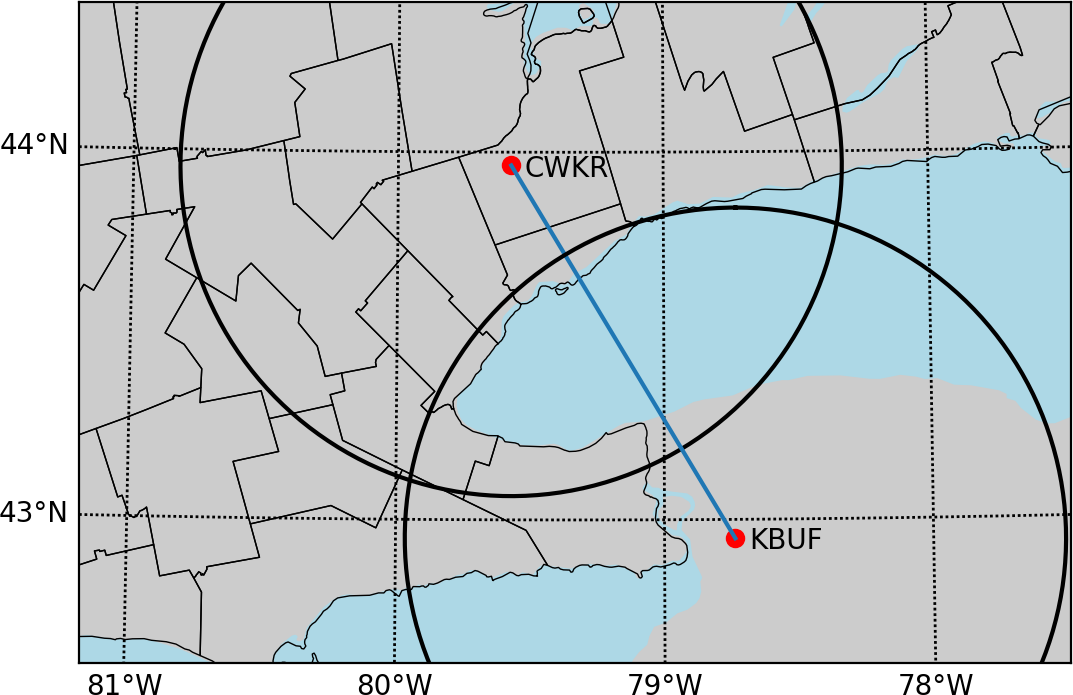
\includegraphics[width=\textwidth]{map}
\caption{The location of the NWS Buffalo Radar (KBUF) and King City Radar (CWKR) are shown as red dots, with a 75 km range ring around each.} 
\label{map}
\end{figure}
Figure \ref{map} shows the geographic location of the radar sites in comparison with each other.

 



